\section{状态访问与不变分布}
\label{sec:dtsp-visits}

多步分布的显式公式~\eqref{eq:dtsp-two-state-power}只对很小的链可得。要判断一般链的长期行为，需要先回答三个更基本的问题：从一个状态出发能到达哪些状态，离开后是否一定回来，以及有没有一个分布被转移完整保持。本节建立这些对象和判别条件；长期分布究竟何时收敛、收敛多快，留到第~\ref{sec:dtsp-long-run}节。前两小节主要处理可数状态集$E$，记$\mathbb P_i,\mathbb E_i$为从$X_0=i$出发时的概率与期望。

\subsection{沟通、周期与回返}
\label{sec:dtsp-communication}

\paragraph{可达与沟通类}
在转移图上，若从$i$出发沿正概率的边能走到$j$，即存在$n\geq0$使$P^n(i,j)>0$，就说$j$从$i$\term{可达}（accessible），记作$i\to j$。若$i\to j$且$j\to i$，称二者\term{沟通}（communicate）。沟通关系自反（取$n=0$）、对称，并且可传递：由$P^{a+b}(i,k)\geq P^a(i,j)P^b(j,k)>0$可知。因此它把$E$分成互不相交的\term{沟通类}（communicating class）。若从一个类出发一步也离不开该类，即对类内的$i$有$\sum_{j\in C}P_{i,j}=1$，称$C$为\term{封闭类}（closed class）。整个状态集构成一个沟通类时，称链满足\term{不可约性}（irreducibility）。

图~\ref{fig:dtsp-communicating-classes}给出一个六状态的例子。状态$1,2$相互沟通，但能流向$3$或$5$，一旦离开就回不来；$\{3,4\}$和$\{5,6\}$都是封闭类。长期看，链最终会落入某个封闭类并永远留在那里，起点决定的只是落入哪一个类的概率。这说明“长期分布”首先取决于类结构：可约链的长期行为一般依赖初态。

\begin{figure}[htbp]
  \centering
  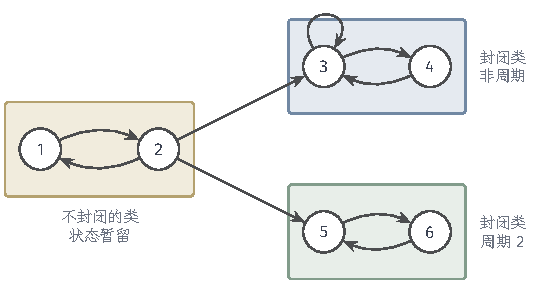
\includegraphics[width=91mm]{figures/03-optimization-evolution-and-signals/02-processes-and-trajectory-evolution/tikz/dtsp-communicating-classes/figure.pdf}
  \caption{六状态链的沟通类。箭头表示一步正概率转移（数值省略）。黄色框$\{1,2\}$不是封闭类，可以经状态$2$离开，其中状态暂留；蓝色框$\{3,4\}$与绿色框$\{5,6\}$都是封闭类，前者因状态$3$的自环而非周期，后者在$5,6$之间确定交替，周期为$2$。}
  \label{fig:dtsp-communicating-classes}
\end{figure}

\paragraph{周期}
即使所有状态互相可达，返回的时刻也可能受到限制。图~\ref{fig:dtsp-communicating-classes}的$\{5,6\}$中，从$5$出发只能在偶数步回到$5$。设$R_i=\{n\geq1:P^n(i,i)>0\}$非空，定义状态$i$的\term{周期}（period）为$d_i=\gcd R_i$。周期为$1$的状态称为非周期的。

周期是沟通类的共同性质。设$i,j$沟通，取$a,b$使$P^a(i,j)>0$、$P^b(j,i)>0$。先走$a$步到$j$再走$b$步回来，说明$a+b\in R_i$；若再在$j$处插入一段长为$n\in R_j$的回路，又有$a+n+b\in R_i$。$d_i$同时整除$a+b$与$a+n+b$，故整除每个$n\in R_j$，从而$d_i\mid d_j$。交换$i,j$得到$d_j\mid d_i$，所以$d_i=d_j$。于是可以说不可约链的周期；周期为$1$时称链是\term{非周期的}（aperiodic）。

周期链的逐时刻分布可能永远振荡。最简单的例子是确定交替链$\bm P=\left(\begin{smallmatrix}0&1\\1&0\end{smallmatrix}\right)$：每一步都合法，从状态$1$出发时$\mathbb P(X_n=2)$在$0$与$1$之间交替，见图~\ref{fig:dtsp-two-state-distribution}(b)。但同一幅图中的时间平均却趋于$1/2$。这一对照提示我们，“分布收敛”和“平均收敛”需要不同的条件；在每个状态加一个停留概率（例如改用$\frac12(\bm I+\bm P)$）就能消除周期。

\paragraph{返回概率与常返}
下面研究离开一个状态后是否一定回来。令
\[
  T_i^{+}=\inf\{n\geq1:X_n=i\},\qquad f_i=\mathbb P_i(T_i^{+}<\infty),
\]
约定空集的下确界为$\infty$。若$f_i=1$，称$i$为\term{常返状态}（recurrent state）；若$f_i<1$，称$i$为\term{暂留状态}（transient state）。

返回概率决定访问次数的分布。记$N_i=\sum_{n\geq0}\mathbb I\{X_n=i\}$为访问$i$的总次数（含时刻$0$）。每次回到$i$后，链“从$i$重新开始”，下一次能否回来与过去无关，所以
\begin{equation}
  \mathbb P_i(N_i>k)=f_i^{k},\qquad k\geq0.
  \label{eq:dtsp-visit-geometric}
\end{equation}
这里在随机的返回时刻重新开始，需要比定义~\ref{def:dtsp-markov-property}更强的强Markov性质，它将在第~\ref{sec:dtsp-strong-markov}节证明。承认这一点，常返等价于访问无穷多次，暂留时$N_i$服从几何分布，$\mathbb E_iN_i=1/(1-f_i)$。另一方面，按定义交换求和与期望，
$\mathbb E_iN_i=\sum_{n\geq0}P^n(i,i)$。两式合起来就得到一个只用转移概率的判别法：

\begin{theorem}[常返的级数判别]
  \label{thm:dtsp-recurrence-series}
  可数状态时间齐次Markov链的状态$i$常返，当且仅当$\sum_{n\geq0}P^n(i,i)=\infty$。若$i$与$j$沟通，则二者同为常返或同为暂留。
\end{theorem}

\begin{proof}
第一句由$\mathbb E_iN_i=\sum_nP^n(i,i)$与式~\eqref{eq:dtsp-visit-geometric}直接得到：$f_i<1$时期望有限，$f_i=1$时$N_i=\infty$几乎必然。对第二句，取$a,b$使$P^a(i,j)>0$、$P^b(j,i)>0$，则$P^{a+n+b}(j,j)\geq P^b(j,i)P^n(i,i)P^a(i,j)$。若$\sum_nP^n(i,i)=\infty$，右侧对$n$求和发散，所以$j$也常返；交换角色得到另一方向。
\end{proof}

\begin{example}[整数格点上的随机游走]
  \label{ex:dtsp-walk-recurrence}
  设$X_{n+1}=X_n\pm1$，向右概率为$p$，向左为$q=1-p$。回到原点必须左右步数相等，所以$P^{2n}(0,0)=\binom{2n}{n}p^nq^n$，奇数步为零。由Stirling公式，$\binom{2n}{n}\sim4^n/\sqrt{\pi n}$，因此
  \[
    P^{2n}(0,0)\sim\frac{(4pq)^n}{\sqrt{\pi n}}.
  \]
  $p=1/2$时$4pq=1$，级数如$\sum n^{-1/2}$发散，原点常返；$p\neq1/2$时$4pq<1$，级数按几何速度收敛，原点暂留。直观上，有漂移的游走以线性速度远离原点，只能回来有限次。
\end{example}

\paragraph{有限封闭类必然常返}
对有限状态链，常返性可以直接由结构判断。设$C$是有限封闭类，固定$i\in C$。对类内每个状态$j$选一条通往$i$的正概率路径；状态有限，所以存在整数$M$和$\varepsilon>0$，使从$C$中任一状态出发，在接下来$M$步内访问$i$的概率至少为$\varepsilon$。按长度为$M$的时间块反复使用Markov性质，得到
\begin{equation}
  \mathbb P_i(T_i^{+}>kM)\leq(1-\varepsilon)^k,\qquad
  \mathbb E_iT_i^{+}=\sum_{n\geq0}\mathbb P_i(T_i^{+}>n)\leq\frac{M}{\varepsilon}<\infty.
  \label{eq:dtsp-finite-return-bound}
\end{equation}
所以有限封闭类中的状态都常返，而且平均返回时间有限。不封闭的类则一定暂留：从中能以正概率走到不能返回的地方。

\paragraph{正常返与零常返}
常返只保证回来，不保证回来得快。记平均返回时间$m_i=\mathbb E_iT_i^{+}$。常返且$m_i<\infty$称\term{正常返}（positive recurrent），常返而$m_i=\infty$称\term{零常返}（null recurrent）。有限封闭类由式~\eqref{eq:dtsp-finite-return-bound}是正常返的；例~\ref{ex:dtsp-walk-recurrence}中的对称游走则是零常返，第~\ref{sec:dtsp-optional-sampling}节将用停时计算证明它从$1$首次到达$0$的期望时间为无穷。两者的差别会在长期平均中显现：第~\ref{sec:dtsp-ergodic-averages}节将证明，正常返状态$i$在长期中被访问的时间比例是$1/m_i$，零常返状态的这一比例为零。

\paragraph{一般状态空间的回返}
状态连续时，单点通常被访问的概率为零，“每个状态互相可达”不再合适，需要换成“每个有正质量的集合都能到达”。固定$(E,\mathcal E)$上的非零测度$\varphi$。若对每个满足$\varphi(B)>0$的$B$和每个初态$x$，链都以正概率在有限时间内进入$B$，称链是$\varphi$不可约的。在此基础上，\term{Harris常返性}（Harris recurrence）要求每个这样的$B$都从每个初态出发几乎必然被访问无穷多次；若再存在不变概率分布，称为\term{正Harris常返性}（positive Harris recurrence）。“以正概率到达”与“几乎必然无穷多次访问”是不同的要求：前者仍允许链以正概率逃离后永不返回。第~\ref{sec:dtsp-long-run}节的一般状态空间结论都以这类回返条件为入口\scite{math-meyn2009markov}。

\subsection{不变分布与平衡方程}
\label{sec:dtsp-invariant}

\paragraph{分布更新的不动点}
第~\ref{sec:dtsp-kernels}节把一步转移写成分布到分布的映射$\mu\mapsto\mu P$。长期问题的第一个候选答案是这个映射的不动点：从它出发走一步，各事件的概率都不变。注意不动的是分布，不是单条路径；路径仍在不停跳动，只是整体比例保持。

\begin{definition}[不变分布]
  \label{def:dtsp-invariant-distribution}
  转移核$P$的概率测度$\pi$若满足$\pi P=\pi$，即
  \[
    \pi(B)=\int_EP(x,B)\,\pi(\mathrm dx),\qquad B\in\mathcal E,
  \]
  则称$\pi$为$P$的\term{不变分布}（invariant distribution），也称\term{平稳分布}（stationary distribution）。满足同一方程、但总质量可以无穷的非负测度称为不变测度。
\end{definition}

有限状态时，不变分布是线性方程组$\bm\pi^{\top}(\bm I-\bm P)=\bm0^{\top}$在约束$\pi_i\geq0$、$\sum_i\pi_i=1$下的解，方程组的每一行说明流入状态$j$的总概率等于$j$原有的概率。对两状态链~\eqref{eq:dtsp-two-state-matrix}，第一行化为$0.1\pi_1=0.2\pi_2$，再归一化得$\bm\pi=(2/3,1/3)$，与式~\eqref{eq:dtsp-two-state-power}的第一项一致。对三状态链
\[
  \bm P=\begin{pmatrix}1/2&1/2&0\\1/4&1/2&1/4\\0&1/2&1/2\end{pmatrix},
\]
解得$\bm\pi=(1/4,1/2,1/4)$；例如第二列给出$\frac14\cdot\frac12+\frac12\cdot\frac12+\frac14\cdot\frac12=\frac12$。

非负与归一化两项条件都不可省略。对例~\ref{ex:dtsp-walk-recurrence}中的对称游走，计数测度$\pi_i=1$满足$\pi P=\pi$，因为每个格点从两侧各接收$1/2$；但它总质量无穷，不能归一化，所以对称游走没有不变分布。可约链的平衡方程又可能有多维解空间，其中包含正负相消的向量，它们满足方程却不是分布。

\paragraph{存在与唯一}
下面的定理回答有限链何时有、以及只有一个不变分布。

\begin{theorem}[有限链的不变分布]
  \label{thm:dtsp-finite-invariant}
  有限状态转移矩阵$\bm P$至少有一个不变分布。若$\bm P$不可约，则不变分布唯一，且每个分量都严格为正。
\end{theorem}

\begin{proof}
存在性：任取初始概率向量$\bm\nu$，考虑Ces\`aro平均$\bm a_n^{\top}=n^{-1}\sum_{k=0}^{n-1}\bm\nu^{\top}\bm P^k$。它们都在有限维概率单纯形中，单纯形是紧集，所以有收敛子列$\bm a_{n_\ell}\to\bm\pi$。又
\[
  \bm a_n^{\top}\bm P-\bm a_n^{\top}=\frac{\bm\nu^{\top}\bm P^n-\bm\nu^{\top}}{n},
\]
其各分量绝对值不超过$2/n$，沿子列取极限得到$\bm\pi^{\top}\bm P=\bm\pi^{\top}$。

正性：设$\bm\pi$是非零非负的不变向量而$\pi_j=0$。由$\pi_j=\sum_i\pi_iP^n(i,j)$，凡能在若干步到达$j$的状态$i$都必须有$\pi_i=0$。不可约时所有状态都能到达$j$，于是$\bm\pi=\bm0$，矛盾。

唯一性：设$\bm\pi,\bm\rho$都是不变分布，令$c=\min_j\pi_j/\rho_j>0$。向量$\bm\pi-c\bm\rho$满足平衡方程、非负，并且至少有一个分量为零；由正性的论证它只能是零向量。两边求和得$c=1$，所以$\bm\pi=\bm\rho$。
\end{proof}

可数状态的不可约链情况更细：不变分布存在当且仅当链是正常返的，此时它唯一，并且$\pi_i=1/m_i$。有限情形的这个公式将在第~\ref{sec:dtsp-ergodic-averages}节由返回分段直接证明；一般可数情形的证明思路相同\scite{math-kallenberg2021probability}。对称游走零常返，与上面“计数测度不能归一化”的观察一致。

\paragraph{存在、唯一与收敛是三件事}
不变分布回答“什么分布被保持”，并没有回答“从别处出发能否到达它”。两个例子把这几件事分开。恒等转移$\bm P=\bm I$保持每一个分布，不变分布不唯一，而且链永远不忘记初态。确定交替链不可约，唯一的不变分布是$(1/2,1/2)$，但从状态$1$出发时逐时刻分布永远在两点间交替，见图~\ref{fig:dtsp-two-state-distribution}(b)。因此在存在与唯一之外，还要有额外条件才能让初态影响消退；第~\ref{sec:dtsp-distribution-convergence}节将证明非周期性正是有限链所缺的那一项。

\subsection{可逆性与细致平衡}
\label{sec:dtsp-reversibility}

\paragraph{正放与倒放}
设想把一条从不变分布启动的链拍成录像，然后倒着播放。对两状态链，倒放的录像与正放在统计上无法区分吗？要回答这个问题，比较正向与反向路径的概率。若对每个$n$，$(X_0,X_1,\ldots,X_n)$与$(X_n,X_{n-1},\ldots,X_0)$同分布，称平稳链是\term{可逆的}（reversible）。取$n=1$，可逆性要求$\mathbb P(X_0=i,X_1=j)=\mathbb P(X_0=j,X_1=i)$，也就是从$i$流向$j$的概率流量等于反向流量。这一条件有自己的名字。

\begin{definition}[细致平衡]
  \label{def:dtsp-detailed-balance}
  概率测度$\pi$与转移核$P$满足\term{细致平衡}（detailed balance），若$E\times E$上的两个测度相等：
  \begin{equation}
    \pi(\mathrm dx)P(x,\mathrm dy)=\pi(\mathrm dy)P(y,\mathrm dx).
    \label{eq:dtsp-detailed-balance}
  \end{equation}
  可数状态时它化为$\pi_iP_{i,j}=\pi_jP_{j,i}$对所有$i,j$成立。
\end{definition}

\begin{theorem}[细致平衡、不变性与可逆性]
  \label{thm:dtsp-detailed-balance}
  若$\pi$与$P$满足细致平衡，则$\pi$是$P$的不变分布，并且从$\pi$启动的链是可逆的。反之，可逆的平稳链满足细致平衡。
\end{theorem}

\begin{proof}
对式~\eqref{eq:dtsp-detailed-balance}在$x\in E$上积分，左侧得$(\pi P)(\mathrm dy)$，右侧得$\pi(\mathrm dy)P(y,E)=\pi(\mathrm dy)$，所以$\pi P=\pi$。可数状态下验证可逆性：由式~\eqref{eq:dtsp-path-probability}，
\[
  \begin{aligned}
    \pi_{i_0}P_{i_0,i_1}P_{i_1,i_2}\cdots P_{i_{n-1},i_n}
    &=P_{i_1,i_0}\,\pi_{i_1}P_{i_1,i_2}\cdots P_{i_{n-1},i_n}\\
    &=\cdots
    =\pi_{i_n}P_{i_n,i_{n-1}}\cdots P_{i_1,i_0},
  \end{aligned}
\]
每一步用一次细致平衡把$\pi$向右移动一格。左端是正向路径的概率，右端是反向路径的概率。一般状态空间用同样的逐步换序处理有限维分布。反方向已由$n=1$的情形说明。
\end{proof}

细致平衡是一组逐对的局部等式，比整体平衡方程容易验证，也容易用来设计转移。两状态链满足它：两条跨状态流量都是$\frac23\times0.1=\frac13\times0.2=\frac1{15}$。上面的三状态链也满足它，每条边两方向的流量都是$1/8$，见图~\ref{fig:dtsp-balance-cycles}(a)。更一般地，在带非负对称边权$w_{i,j}$的图上按$P_{i,j}=w_{i,j}/w_i$随机行走（$w_i=\sum_jw_{i,j}$），取$\pi_i\propto w_i$，便有$\pi_iP_{i,j}\propto w_{i,j}=w_{j,i}\propto\pi_jP_{j,i}$，所以加权图上的随机游走都是可逆的。

\paragraph{平衡不等于细致平衡}
不变分布只要求每个状态的流入总量等于流出总量，并不要求逐边对消。图~\ref{fig:dtsp-balance-cycles}(b)中的三个状态排成一个有向环，每步以$2/3$的概率前进、以$1/3$的概率停留。均匀分布是不变的，因为每个状态从前一个状态接收$\frac13\times\frac23=\frac29$，同时向下一个状态送出同样多；但反方向的流量为零，细致平衡不成立。倒放这条链的录像，会看到它朝相反方向绕圈，一眼就能分辨。

\begin{figure}[htbp]
  \centering
  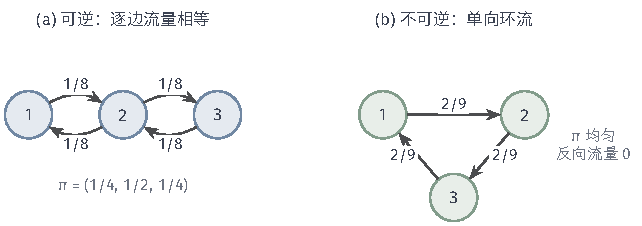
\includegraphics[width=107mm]{figures/03-optimization-evolution-and-signals/02-processes-and-trajectory-evolution/tikz/dtsp-balance-cycles/figure.pdf}
  \caption{细致平衡与整体平衡。边上的数字是平稳运行时一步的概率流量$\pi_iP_{i,j}$。(a)三状态生灭链，$\pi=(1/4,1/2,1/4)$，每条边正反流量都是$1/8$；(b)有向三循环，每步以$2/3$前进、以$1/3$停留（停留流量未画出），均匀分布不变，但只有单向流量$2/9$。}
  \label{fig:dtsp-balance-cycles}
\end{figure}

环路给出一个检验细致平衡的必要条件。若$\pi_iP_{i,j}=\pi_jP_{j,i}$对环路$1\to2\to3\to1$的三条边都成立，把三式相乘、约去$\pi_1\pi_2\pi_3$，就得到$P_{1,2}P_{2,3}P_{3,1}=P_{1,3}P_{3,2}P_{2,1}$：沿环路正走与反走的概率乘积必须相等。有向环中左侧为$(2/3)^3$，右侧为零，所以它不可逆。可逆性因此是一种额外结构，而不是不变分布的必然伴随物。第~\ref{sec:dtsp-mcmc}节将利用细致平衡这一容易验证的充分条件，设计以指定分布为不变分布的采样链。
